\documentclass{beamer}
\usepackage{tikz}
\usepackage{gillius}
\usepackage{abraces}
\usepackage{etex}
\usepackage{array}
\usepackage{multirow}
\usepackage[backend=biber, style=numeric-comp, sorting=none]{biblatex}
\usepackage{hyperref}

% http://tex.stackexchange.com/questions/12703/how-to-create-fixed-width-table-columns-with-text-raggedright-centered-raggedlef
\newcolumntype{L}[1]{>{\raggedright\let\newline\\\arraybackslash\hspace{0pt}}m{#1}}
\newcolumntype{C}[1]{>{\centering\let\newline\\\arraybackslash\hspace{0pt}}m{#1}}
\newcolumntype{R}[1]{>{\raggedleft\let\newline\\\arraybackslash\hspace{0pt}}m{#1}}

\usetikzlibrary{external}
\usetikzlibrary{shapes}
\usetikzlibrary{arrows}
\usetikzlibrary{positioning}
\usetikzlibrary{decorations.pathreplacing}
\usetikzlibrary{calc}

\usetheme[everytitleformat=regular]{m}
%\setbeamertemplate{navigation symbols}{}

\graphicspath{{../figures/}}
\newcommand{\tablepath}{../tables}

\title{Phylogenetic inference of contact network parameters with approximate Bayesian computation}
\author[RMM \& AFYP]{Rosemary M McCloskey$^1$ \and Bioinformatics Training Program \\ Supervisor: Art FY Poon$^{1,2}$}
\institute[UBC \& BCCfE]{$^1$BC Centre for Excellence in HIV/AIDS, Vancouver, Canada \\ $^2$Department of Medicine, University of British Columbia, Vancouver, Canada}
\date{M.Sc. Defence, July 26, 2016}

\newcommand{\dd}[2]{\frac{\text{d}\,#1}{\text{d}\,#2}}

\addbibresource{papers.bib}

\begin{document}
\setbeamercolor{background canvas}{bg=white}
\renewcommand{\footnotesize}{\tiny}
\definecolor{red}{RGB}{228,26,28}
\definecolor{blue}{RGB}{55,126,184}
\definecolor{green}{RGB}{77,175,74}
\definecolor{purple}{RGB}{152,78,163}

\maketitle

%\begin{frame}{Outline}
%    \tableofcontents
%\end{frame}

%\section{Background and Motivation}
%\documentclass{article}
\usepackage{tikz}
\usepackage[T1]{fontenc}
\usepackage[default]{gillius}

\usetikzlibrary{positioning}
\usetikzlibrary{calc}
\usetikzlibrary{arrows}
\usetikzlibrary{automata}

\begin{document}
\pagestyle{empty}

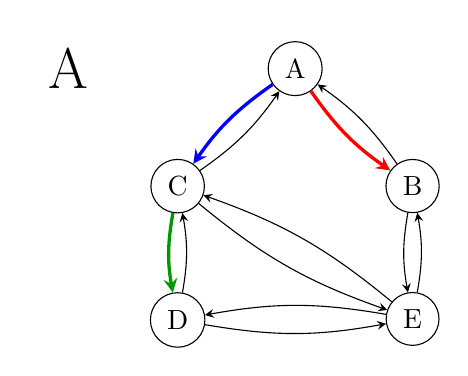
\begin{tikzpicture}
  [every node/.style = {circle, draw},
   every path/.style = {bend right=10, ->, >=stealth}]
  \node (a) {A};
  \node (b) [below right=of a] {B};
  \node (c) [below left=of a] {C};
  \node (d) [below=of c] {D};
  \node (e) [below=of b] {E};

  \node [left=2cm of a, draw=none] {\huge{A}};
  
  \draw (a) [red, very thick] to (b);
  \draw (b) to (a);
  \draw (a) [blue, very thick] to (c);
  \draw (c) to (a);
  \draw (c) to (e);
  \draw (e) to (c);
  \draw (b) to (e);
  \draw (e) to (b);
  \draw (c) [green!60!black, very thick] to (d);
  \draw (d) to (c);
  \draw (d) to (e);
  \draw (e) to (d);
\end{tikzpicture}
\hspace{1cm}
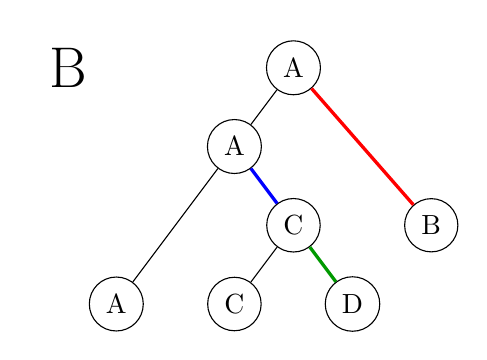
\begin{tikzpicture}
  [every node/.style = {circle, draw}]
  \node (a) at (0, 0) {A};
  \node (c) at (1.5, 0) {C};
  \node (d) at (3, 0) {D};
  \node (b) at (4, 1) {B};

  \node (cd) at (2.25, 1) {C};
  \node (acd) at (1.5, 2) {A};
  \node (abcd) at (2.25, 3) {A};

  \node [left=2cm of abcd, draw=none] {\huge{B}};

  \draw [red, very thick] (abcd) -- (b);
  \draw (abcd) -- (acd);
  \draw [blue, very thick] (acd) -- (cd);
  \draw (acd) -- (a);
  \draw (cd) -- (c);
  \draw [green!60!black, very thick] (cd) -- (d);
\end{tikzpicture}

\end{document}

%\begin{frame}{Viral phylogenies relate individuals' viral genotypes}
  \begin{center}
    \begin{tikzpicture}[
        every node/.style = {inner sep=0pt},
        every path/.style = {-, very thick},
        label/.style = {anchor=south, color=white, inner sep=4pt}
      ]
      \def\pht{1cm}

      \coordinate (abcd);
      \coordinate [below right=1 and 1 of abcd] (b);
      \coordinate [above left=1 and 0.25 of abcd] (acd);
      \coordinate [above left=1 and 0.25 of acd] (a);
      \coordinate [right=of acd] (cd);
      \coordinate [right=1.5 of cd] (c);
      \coordinate [above right=of cd] (d);

      \node (x) [right=0.5 of b, anchor=west, opacity=0.4] {\includegraphics[height=\pht]{stock/person}}; 
      \node (v) at (x.south west) {
\includegraphics[height=\pht]{stock/virus}}; 
      \node at (v.center) {\large b};

      \draw (abcd) -- (acd);
      \draw (abcd) -- (b);

      \node (x) [above=0.7 of a, anchor=south west, opacity=0.4] {\includegraphics[height=\pht]{stock/person}};
      \node (va) at (x.south west) {
\includegraphics[height=\pht]{stock/virus}};
      \node at (va.center) {\large a};
      
      \draw (acd) -- (cd);
      \draw (acd) -- (a);

      \node (x) [above right=0 and 0.8 of c, opacity=0.4] {\includegraphics[height=\pht]{stock/person}};
      \node (v) at (x.south west) {
\includegraphics[height=\pht]{stock/virus}};
      \node at (v.center) {\large c};

      \node (x) [above right=0.8 of d, opacity=0.4] {\includegraphics[height=\pht]{stock/person}};
      \node (v) at (x.south west) {
\includegraphics[height=\pht]{stock/virus}};
      \node at (v.center) {\large d};
      
      \draw (cd) -- (c);
      \draw (cd) -- (d);

      \uncover<2->{
        \node (t1) [below left=of a, inner ysep=6pt] {viruses within individuals};
        \draw [->, >=stealth] (t1.north) -- (va.south west);
      }

      \uncover<3->{
        \node (t2) [below=of t1, inner ysep=6pt] {evolutionary relationships};
        \coordinate [left=0.5 of abcd] (tmp);
        \draw [->, >=stealth] (t2.north) -- (tmp);
      }

    \end{tikzpicture}
  \end{center}
\end{frame}

%\begin{frame}{Transmission trees connect networks to viral phylogenies}
    \begin{tikzpicture}
      [
        every path/.style={very thick, ->, >=stealth}
      ]
      \uncover<1-2>{
        \node (a) at (0, 0) [anchor=center] {\includegraphics[width=\textwidth, trim=0 0 5cm 0, clip]{objects}};
        \node [below=0 of a] {contact network \qquad transmission tree \qquad viral phylogeny};
      }
      \only<1>{ 
        \fill [white] (-1.6, 2.1) rectangle (2.4, -2.7); 
      }
    \end{tikzpicture}
\end{frame}


%\documentclass[landscape]{article}
\usepackage{tikz}
\usepackage[T1]{fontenc}
\usepackage{mathptmx}
\usepackage{fullpage}

\usetikzlibrary{positioning}
\usetikzlibrary{calc}
\usetikzlibrary{arrows}
\usetikzlibrary{automata}

\graphicspath{{stock/}}

\begin{document}
\pagestyle{empty}

\begin{tikzpicture}
  [every node/.style = {inner sep=0pt},
   every path/.style = {->, >=stealth, very thick},
   label/.style = {anchor=south, color=white, inner sep=6pt},
   time/.style = {anchor=north west, inner sep=2pt}]
  \def\pht{1.5cm}
  \def\pd{0.5cm}
  \def\nd{1cm}

  \node (abc) {\includegraphics[height=\pht]{person}};
  \node at (abc.south) [label] {\huge a};

  \node (ac) [below left=\pd of abc] {\includegraphics[height=\pht]{person}};
  \node at (ac.south) [label] {\huge a};

  \node (a) [below left=\pd of ac] {\includegraphics[height=\pht]{person}};
  \node at (a.south) [label] {\huge a};
  \node (b) [below right=\pd of abc] {\includegraphics[height=\pht]{person}};
  \node at (b.south) [label] {\huge b};
  \node (c) [below right=\pd of ac] {\includegraphics[height=\pht]{person}};
  \node at (c.south) [label] {\huge c};

  \draw [red] (abc) -- (b);
  \draw [-, dashed] (abc) -- (ac);
  \draw [blue] (ac) -- (c);
  \draw [-, dashed] (ac) -- (a);

  %\node (a) [left=7cm of abc] {\includegraphics[height=\pht]{person}};
  %\node at (a.south) [label] {\huge a};
  %\node (b) [below left=\nd of a] {\includegraphics[height=\pht]{person}};
  %\node at (b.south) [label] {\huge b};
  %\node (c) [below right=\nd of a] {\includegraphics[height=\pht]{person}};
  %\node at (c.south) [label] {\huge c};
  
  %\draw [red] (a) -- (b);
  %\draw [blue] (a) -- (c);

  \node [below=6cm of abc] (abc) {\includegraphics[height=\pht]{person}};
  \node at (abc.south) [label] {\huge b};

  \node (ac) [below left=\pd of abc] {\includegraphics[height=\pht]{person}};
  \node at (ac.south) [label] {\huge c};

  \node (a) [below left=\pd of ac] {\includegraphics[height=\pht]{person}};
  \node at (a.south) [label] {\huge a};
  \node (b) [below right=\pd of abc] {\includegraphics[height=\pht]{person}};
  \node at (b.south) [label] {\huge b};
  \node (c) [below right=\pd of ac] {\includegraphics[height=\pht]{person}};
  \node at (c.south) [label] {\huge c};

  \draw [-, dashed] (abc) -- (b);
  \draw [green!60!black] (abc) -- (ac);
  \draw [-, dashed] (ac) -- (c);
  \draw [cyan] (ac) -- (a);

  %\node (a) [left=7cm of abc] {\includegraphics[height=\pht]{person}};
  %\node at (a.south) [label] {\huge a};
  %\node (b) [below left=\nd of a] {\includegraphics[height=\pht]{person}};
  %\node at (b.south) [label] {\huge b};
  %\node (c) [below right=\nd of a] {\includegraphics[height=\pht]{person}};
  %\node at (c.south) [label] {\huge c};

  %\draw [green!60!black] (b) -- (c);
  %\draw [cyan] (c) -- (a);

  \node [above left=2cm and 8cm of abc] (abc) {\includegraphics[height=\pht]{person}};
  \node (ac) [below left=\pd of abc] {\includegraphics[height=\pht]{person}};

  \node (a) [below left=\pd of ac] {\includegraphics[height=\pht]{person}};
  \node at (a.south) [label] {\huge a};
  \node (b) [below right=\pd of abc] {\includegraphics[height=\pht]{person}};
  \node at (b.south) [label] {\huge b};
  \node (c) [below right=\pd of ac] {\includegraphics[height=\pht]{person}};
  \node at (c.south) [label] {\huge c};

  \draw [-] (abc) -- (b);
  \draw [-] (abc) -- (ac);
  \draw [-] (ac) -- (c);
  \draw [-] (ac) -- (a);

  %\node (a) [left=7cm of abc] {\includegraphics[height=\pht]{person}};
  %\node at (a.south) [label] {\huge a};
  %\node (b) [below left=\nd of a] {\includegraphics[height=\pht]{person}};
  %\node at (b.south) [label] {\huge b};
  %\node (c) [below right=\nd of a] {\includegraphics[height=\pht]{person}};
  %\node at (c.south) [label] {\huge c};

\end{tikzpicture}
\end{document}

%\begin{frame}{Transmission trees shape viral phylogenies}
  \begin{center}
    \begin{tikzpicture}[
        every node/.style = {inner sep=0pt},
        every path/.style = {->, >=stealth, very thick},
        label/.style = {anchor=south, color=white, inner sep=4pt}
      ]
      \def\pht{1cm}
      \node (abcd) {\includegraphics[height=\pht]{stock/person}};
      \node at (abcd.south) [label] {\Large a};

      \uncover<2>{
      \node (b) at (abcd.east) [anchor=west] {\includegraphics[height=\pht]{stock/person}};
      \node at (b.south) [label] {\Large b};
      \draw [red] (abcd.south) to [bend right=75] (b.south);
      }

      \uncover<3->{
      \node (b) [below right=1 and 0.75 of abcd] {\includegraphics[height=\pht]{stock/person}};
      \node at (b.south) [label] {\Large b};
      \node (acd) [below left=1 and 0.5 of abcd] {\includegraphics[height=\pht]{stock/person}};
      \node at (acd.south) [label] {\Large a};
      \draw [red] (abcd) -- (b);
      \draw [-, dashed] (abcd) -- (acd);
      }

      \uncover<4>{
      \node (cd) at (acd.east) [anchor=west] {\includegraphics[height=\pht]{stock/person}};
      \node at (cd.south) [label] {\Large c};
      \draw [blue] (acd.south) to [bend right=75] (cd.south);
      }
      
      \uncover<5->{
      \node (cd) [below right=0.5 and 0.5 of acd] {\includegraphics[height=\pht]{stock/person}};
      \node at (cd.south) [label] {\Large c};
      \node (a) [below left=0.25 and 0.25 of acd] {\includegraphics[height=\pht]{stock/person}};
      \node at (a.south) [label] {\Large a};
      \draw [blue] (acd) -- (cd);
      \draw [-, dashed] (acd) -- (a);
      }

      \uncover<6>{
      \node (d) at (cd.east) [anchor=west] {\includegraphics[height=\pht]{stock/person}};
      \node at (d.south) [label] {\Large d};
      \draw [green] (cd.south) to [bend right=75] (d.south);
      }

      \uncover<7->{
      \node (c) [below left=0.25 and 0.25 of cd] {\includegraphics[height=\pht]{stock/person}};
      \node at (c.south) [label] {\Large c};
      \node (d) [below right=0.4 and 0.4 of cd] {\includegraphics[height=\pht]{stock/person}};
      \node at (d.south) [label] {\Large d};
      \draw [-, dashed] (cd) -- (c);
      \draw [green!80!black] (cd) -- (d);
      }

      \coordinate [below right=0.5 and 3 of b] (abcd);
      \coordinate [below right=1 and 1 of abcd] (b);
      \coordinate [above left=1 and 0.25 of abcd] (acd);
      \coordinate [above left=1 and 0.25 of acd] (a);
      \coordinate [right=of acd] (cd);
      \coordinate [right=1.5 of cd] (c);
      \coordinate [above right=of cd] (d);

      \uncover<1-2>{
      \node (x) at (abcd) {
\includegraphics[height=\pht]{stock/virus}};
      \node at (x.center) {\large a};
      }

      \uncover<2>{
      \node (x) [below right=0.3 of abcd, anchor=north west] {
\includegraphics[height=\pht]{stock/virus}}; 
      \node at (x.center) {\large b};
      }

      \uncover<3-4>{
      \node (x) [above=0 of acd, anchor=south] {
\includegraphics[height=\pht]{stock/virus}}; 
      \node at (x.center) {\large a};
      }

      \uncover<3->{
      \node (x) [below right=-0.2 of b, anchor=north west] {
\includegraphics[height=\pht]{stock/virus}}; 
      \node at (x.center) {\large b};

      \draw (abcd) -- (acd);
      \draw (abcd) -- (b);
      }

      \uncover<4>{
      \node (x) [right=0.3 of acd, anchor=west] {
\includegraphics[height=\pht]{stock/virus}}; 
      \node at (x.center) {\large c};
      }

      \uncover<5-6>{
      \node (x) at (cd) [anchor=west] {
\includegraphics[height=\pht]{stock/virus}};  
      \node at (x.center) {\large c};
      }
      
      \uncover<5->{
      \node (x) at (a) [anchor=south] {
\includegraphics[height=\pht]{stock/virus}};
      \node at (x.center) {\large a};
      
      \draw (acd) -- (cd);
      \draw (acd) -- (a);
      }

      \uncover<6>{
      \node (x) [above right=0.4\pht and 0.4\pht of cd] [anchor=south west] {\includegraphics[height=\pht]{stock/virus}};
      \node at (x.center) {\large d};
      }

      \uncover<7->{
      \node (x) at (c) [anchor=west] {\includegraphics[height=\pht]{stock/virus}};
      \node at (x.center) {\large c};

      \node (x) at (d) [anchor=south west] {\includegraphics[height=\pht]{stock/virus}};
      \node at (x.center) {\large d};
      
      \draw (cd) -- (c);
      \draw (cd) -- (d);
      }
    \end{tikzpicture}
  \end{center}
\end{frame}

%\begin{frame}{Can we fit network models from viral sequence data?}
    \begin{tikzpicture}
      [
        every path/.style={very thick, ->, >=stealth}
      ]
      \uncover<2->{
        \node at (0, 0) [anchor=center] {\includegraphics[width=\textwidth]{objects}};
        \draw (-3.5, 2) to [bend left=75] (-1.5, 2);
      }
      \only<2>{ 
        \fill [white] (0, 2) rectangle (6, -2); 
      }
      \only<3>{
        \fill [white] (2.8, 2) rectangle (6, -2); 
      }
      \uncover<3->{
        \draw (-1, 2) to [bend left=75] (1, 2);
      }

      \uncover<4->{
        \draw (1.5, 2) to [bend left=75] (3.5, 2);
      }

      \uncover<5->{
        \draw [green] (3.5, -2) to [bend left=75] node [auto, green] {\Large \checkmark} (1.5, -2);
      }

      \uncover<6->{
        \draw [green] (1, -2) to [bend left=75] node [auto, green] {\Large ``\checkmark''} (-1, -2);
      }
      \uncover<7->{
        \draw [orange] (-1.5, -2) to [bend left=75] node [auto] {\Large \alert{?}} (-3.5, -2);
      }
    \end{tikzpicture}
\end{frame}


%%\begin{frame}{Network models formally describe network structure}
  \begin{columns}
    \column{0.55\textwidth}
    \begin{minipage}[c][.6\textheight][c]{\linewidth}
      \begin{enumerate}
        \setlength{\itemsep}{12pt}
        \uncover<2->{
        \item Start with \only<2-6>{10}\only<7->{\alert{$n$}} women and 
          \only<2-6>{10}\only<7->{\alert{$n$}} men.
        }
        \uncover<3->{
        \item Randomly form \only<3-6>{20}\only<7->{\alert{$p \times n$}} male-female partnerships.
        }
        \uncover<4->{
        \item Randomly rewire each edge with \only<4-6>{10}\only<7->{\\\alert{$q$ }}\% probability.
        }
      \end{enumerate}
    \end{minipage}
    \column{0.5\textwidth}
    \begin{minipage}[c][.6\textheight][c]{\linewidth}
      \only<2>{\includegraphics[width=5cm, page=1]{homophily}}
      \only<3>{\includegraphics[width=5cm, page=2]{homophily}}
      \only<4>{\includegraphics[width=5cm, page=3]{homophily}}
      \only<5->{\includegraphics[width=5cm, page=4]{homophily}}
    \end{minipage}
  \end{columns}

  \vspace{0.5cm}
  \begin{columns}
    \column{0.55\textwidth}
    \uncover<6->{\centerline{\large{network model}}}
    \column{0.55\textwidth}
    \uncover<6->{\centerline{\large{contact network}}}
  \end{columns}
\end{frame}

%\begin{frame}{Why fit network models?}
  \begin{columns}
    \column{0.33\textwidth}
    \uncover<2->{
    \includegraphics[width=0.85\textwidth]{sir-trajectories-vertical}
    }

    \column{0.33\textwidth}
    \uncover<3->{
    \includegraphics[width=0.75\textwidth]{nettypes}
    }

    \column{0.33\textwidth}
    \uncover<4->{
    \begin{tikzpicture}
      \node (pic) { \includegraphics[width=0.75\textwidth]{vaccinate} };
      \node at (pic.east) { \includegraphics[width=1cm]{stock/syringe} };
    \end{tikzpicture}
    }
  \end{columns}

  \begin{columns}
    \column{0.33\textwidth}
    \uncover<2->{
    \centerline{\large predict}
    }

    \column{0.33\textwidth}
    \uncover<3->{
    \centerline{\large characterize}
    }

    \column{0.33\textwidth}
    \uncover<4->{
    \centerline{\large simulate}
    }
  \end{columns}
\end{frame}


%\section{The Barab\'asi-Albert (BA) Contact Network Model}
%\begin{frame}{BA model incorporates preferential attachment}
  \begin{columns}
  \column{0.5\textwidth}
  \begin{tikzpicture}[
      scale=2,
      every edge/.style={thick}
    ]
    \node (n1) at (1, 0) [circle, fill=black] { };
    \node (n2) at (0.86, 0.5) [circle, fill=black] { };
    \node (n3) at (0.5, 0.86) [circle, fill=black] { };
    \draw (n1) -- (n2) -- (n3) -- (n1);

    \uncover<2->{
      \node (n4) at (0, 1) [circle, fill=black] { };
    }
    \only<2-3>{
      \node [right=0 of n4.north east, anchor=south west] {$m = 2$};
    }
    \only<2-4>{
      \draw (n4) -- ++ (0.2, -0.2);
      \draw (n4) -- ++ (-0.2, -0.2);
    }

    \node [right=0 of n1] {%
      \only<3-4>{$2^\alpha+1$}%
      \only<6-7>{$3^\alpha+1$}%
    };
    \node [right=0 of n2] {%
      \only<3-4>{$2^\alpha+1$}%
      \only<6-7>{$3^\alpha+1$}%
    };
    \node [right=0 of n3] {%
      \only<3-4>{$2^\alpha+1$}%
      \only<6-7>{$2^\alpha+1$}%
    };

    \only<4>{
      \draw (n4) -- ++ (0.2, -0.2) -- (n2);
      \draw (n4) -- ++ (-0.2, -0.2) -- (n1);
    }

    \uncover<5->{
      \draw (n4) -- (n2);
      \draw (n4) -- (n1);
    }

    \uncover<6->{
      \node (n5) at (-0.5, 0.86) [circle, fill=black] { };
    }

    \only<6-7> {
      \draw (n5) -- ++ (0.2, -0.2);
      \draw (n5) -- ++ (-0.2, -0.2);
    }
    
    \uncover<6-7>{ \node [right=0 of n4.north east, anchor=south west] { $2^\alpha+1$ }; }

    \only<7>{
      \draw (n5) -- ++ (0.2, -0.2) -- (n3);
      \draw (n5) -- ++ (-0.2, -0.2) -- (n2);
    }

    \uncover<8->{
      \draw (n5) -- (n3);
      \draw (n5) -- (n2);
    }
    
    \uncover<9->{
      \node (n6) at (-0.86, 0.5) [circle, fill=black] { };
      \draw (n6) -- (n2);
      \draw (n6) -- (n1);
    }

    \uncover<10->{
      \node (n7) at (-1, 0) [circle, fill=black] { };
      \draw (n7) -- (n3);
      \draw (n7) -- (n4);
    }

    \uncover<11->{
      \node (n8) at (-0.86, -0.5) [circle, fill=black] { };
      \node (n9) at (-0.5, -0.86) [circle, fill=black] { };
      \node (n10) at (0, -1) [circle, fill=black] { };
      \node (n11) at (0.5, -0.86) [circle, fill=black] { };
      \node (n12) at (0.86, -0.5) [circle, fill=black] { };

      \draw (n8) -- (n2);
      \draw (n8) -- (n4);
      \draw (n9) -- (n2);
      \draw (n9) -- (n1);
      \draw (n10) -- (n2);
      \draw (n10) -- (n8);
      \draw (n11) -- (n3);
      \draw (n11) -- (n9);
      \draw (n12) -- (n2);
      \draw (n12) -- (n8);
    }

    \uncover<12->{
      \node (n1) at (1, 0) [circle, fill=red] { };
      \node (n2) at (0.86, 0.5) [circle, fill=red] { };
      \node (n5) at (-0.86, 0.5) [circle, fill=red] { };
      \node (n7) at (-0.86, -0.5) [circle, fill=red] { };
      \node (n8) at (-0.5, -0.86) [circle, fill=red] { };

      \draw [ultra thick, red] (n2) -- (n7);
      \draw [ultra thick, red] (n2) -- (n1);
      \draw [ultra thick, red] (n8) -- (n1);
      \draw [ultra thick, red] (n5) -- (n2);
    }

    \only<11>{\node [below=of n10] {$N = 12$};}
    \uncover<12->{\node [below=of n10] {$I = 5$};}
  \end{tikzpicture}

  \column{0.4\textwidth}
  \uncover<2->{
    $m$ = number of new edges per vertex \\
    \hfill\\
  }

  \uncover<3->{
    $\alpha$ = preferential attachment power ($\Pr \propto
    \text{degree}^{\alpha} + 1$) \\
    \hfill\\
  }

  \uncover<11->{
    $N$ = number of nodes \\
    \hfill\\
  }

  \uncover<12->{
    $I$ = number of infected nodes (prevalence) 
  }
  \end{columns}
\end{frame}

%\begin{frame}{Are network parameters identifiable from tree shape?}
  \begin{minipage}[p][0.6\textheight][t]{\textwidth}
    \only<2>{\includegraphics[width=0.9\textwidth, trim=0 2.8in 0 0, clip]{kernel-idea.pdf}}
    \only<3>{\includegraphics[width=0.9\textwidth, trim=0 1.7in 0 0, clip]{kernel-idea.pdf}}
    \only<4>{\includegraphics[width=0.9\textwidth, trim=0 0.8in 0 0, clip]{kernel-idea.pdf}}
    \only<5->{\includegraphics[width=0.9\textwidth, trim=0 0in 0 0, clip]{kernel-idea.pdf}}
  \end{minipage}
\end{frame}

%\begin{frame}{yes they are}
  \centerline{\includegraphics[height=0.8\textheight]{kernel-kpca}}
\end{frame}


%\section{\textit{Netabc}: Phylogenetic Reconstruction of Contact Network Parameters with Approximate Bayesian Computation}
%\begin{frame}{Simulated trees can be used to fit network models}
  \centerline{\includegraphics[width=0.9\textwidth]{abc-smc}}

  \centerline{animate this?}
\end{frame}

%\begin{frame}{Marginal posterior distributions for $\alpha$ show least spread}
  \vspace{-0.5cm}
  \begin{tikzpicture}
    \node at (0, 0) [anchor=center] {\includegraphics[trim=1cm 0 0 0, clip, width=0.8\textwidth]{{abc-posterior/1.0_1000_3_5000_0}.pdf}};
    \node at (-4, 3) [anchor=center, text width=2cm, fill=white, inner sep=2pt] {preferential attachment};
    \node at (4.5, 3) [anchor=center, text width=2cm, fill=white, inner sep=2pt] {number infected};
    \node at (-4.2, -1) [anchor=center, text width=2cm, align=center, fill=white, inner ysep=2pt, inner xsep=0pt] {edges per vertex};
    \node at (4.2, -0.7) [anchor=center, text width=1.5cm, align=center, fill=white, inner sep=2pt] {total nodes};

    \only<1>{ \fill [white] (0, 0) rectangle (4.8, 3.8);}
    \only<1-2>{ \fill [white] (0, 0) rectangle (-5, -3.8);}
    \only<1-3>{ \fill [white] (0, 0) rectangle (4.8, -3.8);}
    \only<4>{ }
  \end{tikzpicture}
\end{frame}

%\begin{frame}{Two-dimensional posteriors show parameter correlations}
  \includegraphics[width=\textwidth]{{abc-posterior-2d/1.0_1000_3_5000_0}.pdf}
\end{frame}

%\begin{frame}{$\alpha$ and $I$ are identifiable with ABC}
  \vspace{-0.5cm}
  \begin{tikzpicture}
    \node at (0, 0) [anchor=center] {\includegraphics[width=\textwidth]{abc-boxplot}};
    \only<1> { 
      \fill [white] (-1.2, 0.5) rectangle (2, 3.8);
      \fill [white] (-1.2, -4) rectangle (2, -3);
    }
    \only<1-2> { 
      \fill [white] (2, 0.5) rectangle (6, 3.8); 
      \fill [white] (2, -4) rectangle (6, -3);
    } 
    \only<1-3>{ \fill [white] (-5.5, -3) rectangle (6, 0.5); }
    \only<4>{ }
  \end{tikzpicture}
\end{frame}

%\begin{frame}{$m$ and $N$ are not identifiable with ABC}
  \vspace{-0.5cm}
  \begin{tikzpicture}
    \node at (0, 0) [anchor=center] {\includegraphics[width=\textwidth]{abc-boxplot-mN}};
    \only<1>{ \fill [white] (-5.5, -3) rectangle (6, 0.5); }
    \only<2>{ }
  \end{tikzpicture}
\end{frame}


\section{Application to real HIV epidemics}
\begin{frame}{Application to real world HIV datasets}
  \centerline{\begin{tabular}{ccc}
  Dataset & Sequences ($n$) & Gene \\
  \hline
  IDU/Estonia~\autocite{zetterberg2004two} & 171/188 & \textit{env}/\textit{gag} \\
  IDU/Romania~\autocite{niculescu2015recent} & 136 & \textit{pol} \\
  IDU/Canada & 399 & \textit{pol} \\
  HET/Botswana~\autocite{novitsky2013phylogenetic,novitsky2014impact} & 180 & \textit{env} \\
  HET/Malawi~\autocite{mccormack2002early} & 141/154 & \textit{env}/\textit{gag} \\
  HET/Uganda~\autocite{grabowski2014role} & 225 & \textit{env}/\textit{gag} \\
  MSM/Beijing~\autocite{wang2015targeting} & 173 & \textit{pol} \\
  MSM/Taiwan~\autocite{kao2011surveillance} & 275 & \textit{pol} \\
  MSM/USA~\autocite{little2014using} & 180 & \textit{pol} \\
  MSM/Shanghai~\autocite{li2015hiv} & 280 & \textit{pol} \\
  mixed/Spain~\autocite{cuevas2009hiv} & 287 & \textit{pol} \\
  \hline
\end{tabular}
}
\end{frame}


\section{Conclusions}

\end{document}

\begin{frame}{HIV networks have sub-linear preferential attachment}
    Also, higher PA for IDU networks.

    \includegraphics[trim=0 3.5in 3.3in 0, clip, width=0.5\textwidth]{realdata-hpd-bc}
    \includegraphics[trim=3.4in 1.5in 0 2.0in, clip, width=0.5\textwidth]{realdata-hpd-bc}
\end{frame}

\begin{frame}{Conclusions}
  \begin{itemize}
    \item We developed a phylodynamic method to fit contact network models to
      phylogenetic data.
      \pause
    \item The preferential attachment power of the Barab\'asi-Albert network
      model, which is challenging to estimate by traditional epidemiological
      methods, can be estimated with ABC.
      \pause
    \item The networks underlying real epidemics are heterogeneous,
      underscoring the importance of considering network structure in
      phylodynamic analyses.
  \end{itemize}
\end{frame}

\begin{frame}{Acknowledgements}
  \begin{columns}
    \begin{column}{0.6\textwidth}

      \textbf{BC Centre for Excellence in HIV/AIDS}

      Art Poon

      Jeff Joy

      Richard Liang

      Thuy Nguyen

      P. Richard Harrigan

      \hfill\\
      \textbf{University of British Columbia}

      Sarah Otto

      Alexandre Bouchard-C\^ot\'e

      \vfill
      \vspace{0.5cm}
      $\qquad\qquad$\includegraphics[width=2cm]{logos/genomecanada}
      $\qquad$
      \includegraphics[width=2cm]{logos/genomequebec}
    \end{column}
    \begin{column}{0.4\textwidth}
      \centering 

      \includegraphics[width=3cm]{logos/cfe}
      \vspace{0.5cm}

      \includegraphics[width=3cm]{logos/cihr}

      \includegraphics[width=3cm]{logos/genomebc}

      \includegraphics[width=3cm]{logos/bmgf}
      \vspace{0.5cm}

      \includegraphics[width=3cm]{logos/btp}
    \end{column}
  \end{columns}
\end{frame}

\end{document}
